\documentclass[11pt]{article}

\usepackage[a4paper,margin=1in]{geometry}
\usepackage[T1]{fontenc}
\usepackage[utf8]{inputenc}
\usepackage{lmodern}
\usepackage{microtype}
\usepackage{amsmath,amssymb,amsthm,mathtools,bm}
\usepackage{booktabs}
\usepackage{enumitem}
\usepackage{natbib}
\usepackage{hyperref}
\usepackage{setspace}
\usepackage{graphicx}
\usepackage{float}
\usepackage{caption}

\hypersetup{colorlinks=true,citecolor=blue,linkcolor=blue,urlcolor=blue}
\setstretch{1.06}
\setlength{\emergencystretch}{3em}
\graphicspath{{figures/}}

\newtheorem{proposition}{Proposition}
\newtheorem{lemma}{Lemma}
\newtheorem{remark}{Remark}

\newcommand{\E}{\mathbb{E}}
\newcommand{\Prob}{\mathbb{P}}
\newcommand{\1}{\mathbf{1}}
\newcommand{\R}{\mathbb{R}}
\newcommand{\Mhat}{\hat M}

\title{\bfseries Legitimacy Gating in Social Learning}
\author{Gabriel Bontemps \and Abhishek Banerjee}
\date{June 2026}

\begin{document}
\maketitle

\begin{abstract}
\noindent
Standard models of social learning assume that reward feedback is always valid
evidence: a bad outcome is information that one's belief was wrong. But people
often respond to a bad outcome by questioning the rule that produced it rather
than their own choice. We develop a computational social simulation of
\emph{legitimacy-gated} learning. Agents choose between rewarded actions, but
rewards discipline beliefs only through a latent legitimacy state $L_{i,t}$ that
measures whether the reward rule is accepted as evidence: the effective
prediction error is $L_{i,t}$ times the raw prediction error. Legitimacy depends
on perceived fairness, defined relative to a benchmark for a representative modal
agent; because agents may misrepresent that benchmark, the same rule can be read
as fair by one community and unfair by another. Fairness discomfort is
asymmetric --- disadvantageous unfairness hurts more than advantageous
unfairness --- and only discomfort beyond an acceptability threshold erodes
legitimacy. Network geometry transmits both credibility and fairness benchmarks.
Simulations identify four regimes: legitimate consensus, correct-but-illegitimate
consensus, defensive wrong consensus, and fairness polarisation. The central
finding is that legitimacy collapse converts a \emph{correctable} early error
into a persistent one: a society that would have corrected an early mistake
($93\%$ optimal-arm mass) instead locks onto it ($1\%$) once corrective feedback
loses authority. The model builds on the credibility-transmission mechanism of
\citet{BontempsBanerjee2026} but studies a distinct behavioural layer ---
whether feedback is accepted as legitimate evidence --- and is self-contained.
A replication package regenerates every figure and table.
\end{abstract}

\noindent\textbf{Keywords:} social learning; legitimacy; fairness; reinforcement
learning; reward discounting; community networks; agent-based simulation;
polarisation.

\section{Introduction}
A bad outcome is ambiguous. It can be read as evidence that one's belief was
wrong, or as evidence that the rule assigning outcomes is unfair. Models of
social and reinforcement learning almost always assume the first reading:
realised rewards are valid evidence and prediction errors discipline beliefs
directly \citep{SuttonBarto2018,DeGroot1974,GolubJackson2010}. Yet a large body
of work on fairness, legitimacy and motivated cognition documents the second:
people discount, reinterpret or reject information that conflicts with what they
feel they deserve \citep{Rabin1993Fairness,FehrSchmidt1999,Tyler2006,Kunda1990,Festinger1957}.
This paper asks a simple question: \emph{when do agents stop treating reward
feedback as valid evidence because the reward rule is perceived as unfair, and
how does network geometry shape the result?}

We answer it with a computational social simulation in which the authority of
feedback is itself a learned, social quantity. Each agent carries a latent
\emph{legitimacy} state $L_{i,t}\in[0,1]$ that gates learning: the effective
prediction error is $L_{i,t}$ times the raw prediction error, so that when the
rule is seen as illegitimate, even strong corrective feedback barely moves
beliefs. Legitimacy is not exogenous. It falls when accumulated \emph{fairness
discomfort} exceeds an acceptability threshold and recovers slowly when outcomes
are acceptable. Fairness is judged against a benchmark for a representative
\emph{modal agent}; agents may hold distorted benchmarks, and those benchmarks
are themselves transmitted on the network. Discomfort is asymmetric:
disadvantageous unfairness weighs more than advantageous unfairness.

The point of departure is a credibility-transmission baseline in which confidence
is generated by the decision process and socially transmitted as credibility
\citep{BontempsBanerjee2026}. There, agents can become collectively wrong, but
they never dispute the rule: rewards remain valid evidence. The present paper
relaxes exactly that assumption. The behavioural layer it adds is not who is
believed (credibility) but whether the feedback counts at all (legitimacy). The
two interact: credibility-weighted transmission still spreads actions and
confidence, while a second channel spreads fairness benchmarks, and legitimacy
decides how much realised reward is allowed to teach.

The simulations identify four regimes. In \emph{legitimate consensus} agents
converge on the reward-maximising action with high legitimacy. In
\emph{correct-but-illegitimate consensus} they learn the optimal action but
legitimacy collapses: they know what works yet believe the game is unfair. In
\emph{defensive wrong consensus} they lock onto the wrong action and discount the
corrective feedback that would overturn it. In \emph{fairness polarisation}
communities differ in legitimacy --- and even in action --- under an identical
reward rule, purely because they hold different fairness benchmarks. The headline
result is that legitimacy gating makes wrong consensus \emph{persistent}: a
configuration that corrects an early error when feedback is fully authoritative
instead entrenches it once legitimacy collapses.

\paragraph{Contributions.}
\begin{enumerate}[label=(\roman*),leftmargin=2.2em,itemsep=1pt]
\item A self-contained agent-based model in which reward feedback teaches only
through an endogenous legitimacy gate, with fairness judged against a
transmissible modal-agent benchmark and asymmetric discomfort.
\item Four operational regimes --- legitimate, correct-but-illegitimate,
defensive-wrong, and fairness-polarised --- and an analytical legitimacy-collapse
condition.
\item Six experiments showing asymmetric legitimacy loss, an acceptability
threshold, benchmark-driven fairness polarisation without payoff differences,
legitimacy-gated persistence of wrong consensus, and the role of network
geometry.
\item A replication package (code, tests, configs, scripts) regenerating every
result.
\end{enumerate}

\section{Background and positioning}
\label{sec:background}
The model sits between three literatures. \emph{Social and reinforcement
learning} explains how agents aggregate dispersed information and learn from
reward \citep{DeGroot1974,GolubJackson2010,SuttonBarto2018}, and opinion-dynamics
models explain when interaction yields consensus, clustering or polarisation
\citep{HegselmannKrause2002,FlacheMasEtAl2017}. These models treat the evidential
status of feedback as fixed. \emph{Fairness and inequity aversion} in economics
formalises the idea that agents care about how outcomes compare to a reference,
asymmetrically \citep{Rabin1993Fairness,FehrSchmidt1999,BoltonOckenfels2000,CharnessRabin2002};
we borrow the asymmetric reference-dependent form but place it inside a learning
loop rather than a one-shot utility. Crucially, fairness ideals are
\emph{heterogeneous} --- individuals hold systematically different notions of a
fair reference \citep{CappelenHoleSorensenTungodden2007,Andre2024ShallowMeritocracy}
--- which is the empirical basis for our transmissible, community-specific
benchmark $\hat M$ and the fairness-polarisation regime it generates. Legitimacy
is thus an \emph{endogenous, socially learned norm}, in the tradition of
endogenous preferences and culturally transmitted norms
\citep{Bowles1998,Tyler2006}. \emph{Legitimacy and motivated cognition}
explain why perceived unfairness changes whether a rule is accepted and whether
discordant information is processed \citep{Tyler2006,Kunda1990,Festinger1957}; we
operationalise this as a gate on the prediction error. Neuroeconomically, the gate
is a modulation of the evidential weight of reward prediction errors: social and
non-social learning share prediction-error machinery, and self- versus
other-referenced prediction errors are represented and can be up- or
down-weighted according to context \citep{JoinerPivaTurrinChang2017}. The
legitimacy state is exactly such a context variable, scaling how much a realised
reward is allowed to teach. This places the mechanism inside the current debate
over what orbitofrontal and prefrontal cortex compute --- explicit economic value
\citep{PadoaSchioppaConen2017} versus a latent task-state or cognitive map that
contextualises value updating \citep{HaydenNiv2021}; legitimacy is a
state-like context variable of the second kind. Behaviourally, a
\emph{defensive-wrong} consensus is a failure of \emph{reversal learning} --- the
capacity to overturn a previously reinforced contingency, whose neural substrate
is well characterised \citep{IzquierdoBrigmanRadkeRudebeckHolmes2017} --- brought
about socially rather than by lesion. We connect the resulting regimes to
behavioural-equilibrium theory (Section~\ref{sec:equilibrium}): quantal response
and its regular, axiomatic form
\citep{McKelveyPalfrey1995,GoereeHoltPalfrey2005}, the systematic experimental
anomalies these were built to explain \citep{GoereeHolt2001}, the set-valued
M-equilibrium \citep{GoereeLouis2021}, and nonequilibrium / level-$k$ reasoning
about a modal agent \citep{Nagel1995,CamererHoChong2004,CrawfordCostaGomesIriberri2013};
the learning dynamics themselves are of the reinforcement / experience-weighted
family studied in learning-in-games \citep{ErevRoth1998,CamererHo1999EWA}.

Relative to the credibility-transmission baseline \citep{BontempsBanerjee2026},
the contribution is a different behavioural layer. There, the open question is
whose action is believed; here it is whether the feedback is admitted as
evidence at all. We re-use the credibility backbone (process-based choice,
endogenous confidence, dual-channel social influence on community networks) but
define every component independently, and the new mechanism --- legitimacy
gating with a transmissible fairness benchmark --- is original to this paper.

\section{The model}
\label{sec:model}
Figure~\ref{fig:mechanism} summarises the mechanism. We describe it in ODD+D
terms in Appendix~\ref{app:odd}.

\begin{figure}[t]
\centering
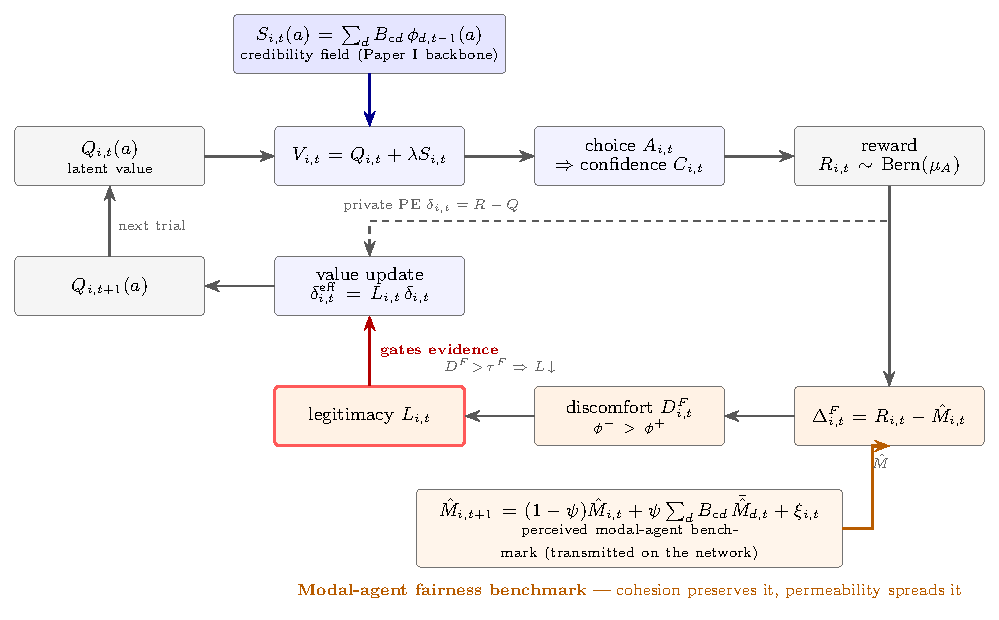
\includegraphics[width=\textwidth]{fig1_mechanism.pdf}
\caption{Mechanism. The value/choice pipeline (top) is the credibility backbone:
augmented values drive a process-based choice and endogenous confidence, and a
credibility field transmits confidence-weighted actions. The reward then enters a
fairness branch (right): the discrepancy from a perceived modal-agent benchmark
$\hat M$ produces asymmetric discomfort, which moves legitimacy $L$ across an
acceptability threshold $\tau^F$. Legitimacy \emph{gates} the prediction error
($\delta^{\mathrm{eff}}=L\,\delta$, red), so illegitimate feedback barely teaches.
The modal-agent benchmark is itself transmitted on the network (bottom).}
\label{fig:mechanism}
\end{figure}

\paragraph{Environment and states.}
Time is discrete, $t\in\mathbb N_0$. Agents $V=\{1,\dots,N\}$ are partitioned into
$M$ communities with row-stochastic coupling matrix $B$ (cohesion $B_{cc}$,
permeability $\Gamma_c=1-B_{cc}$); the induced agent network has balanced block
weights $W_{ij}=B_{cd}/N_d$. Two arms pay Bernoulli rewards with means
$\mu_1,\mu_2$; $a^\star=\arg\max_a\mu_a$. Each agent carries values $Q_{i,t}(a)$,
confidence $C_{i,t}$, legitimacy $L_{i,t}\in[0,1]$, and a perceived modal-agent
fairness benchmark $\hat M_{i,t}\in[0,1]$.

\paragraph{Choice, confidence, credibility.}
The anticipatory credibility field is the confidence-weighted mass of neighbours'
previous actions, $S_{i,t}(a)=\sum_{d}B_{cd}\,\phi_{d,t-1}(a)$ with
$\phi_{c,t}(a)=\frac1{N_c}\sum_{i\in V_c}\1\{A_{i,t}=a\}C_{i,t}$. Augmented values
are $V_{i,t}(a)=Q_{i,t}(a)+\lambda S_{i,t}(a)$, the drift is
$v_{i,t}=\beta(V_{i,t}(1)-V_{i,t}(2))$, and the action follows the exact
symmetric-boundary hitting probability
$\Prob(A_{i,t}=1)=(1+e^{-2v_{i,t}a/\sigma^2})^{-1}$. Confidence is the balance of
evidence, $C_{i,t}=|2\Prob(A_{i,t}=1)-1|\in(0,1)$.

\paragraph{Modal-agent fairness benchmark.}
Fairness is judged against a representative \emph{modal agent}. We distinguish
three objects: the true modal-agent benchmark $M$; agent $i$'s \emph{perceived}
benchmark $\hat M_{i,t}\in[0,1]$; and the perceived fair reward for an action,
$r^F_{i,t}(a)=f(a,\hat M_{i,t})$. The baseline uses the scalar form
$f(a,\hat M)=\hat M$; an effort--reward form
$f(a,\hat M)=b_0+b_1\1\{a=\text{high effort}\}+b_2\hat M$, in which a high-effort
action is expected to deserve more reward, is available behind a configuration
flag and leaves the baseline experiments unchanged. $\hat M_{i,t}$ is the
perceived benchmark reward entitlement of the modal agent under the current rule;
agents may \emph{misrepresent} it ($\hat M_{i,t}\neq M$), and the perceived
benchmark is itself socially learned (Eq.~\ref{eq:Mupdate}).

\paragraph{Fairness discrepancy, discomfort, legitimacy.}
The fairness discrepancy is
\begin{equation}
\Delta^F_{i,t}=R_{i,t}-r^F_{i,t}(A_{i,t}),
\label{eq:dF}
\end{equation}
negative for disadvantageous and positive for advantageous unfairness. Discomfort
is asymmetric,
\begin{equation}
D^F_{i,t}=\phi^-[-\Delta^F_{i,t}]_+ + \phi^+[\Delta^F_{i,t}]_+,
\qquad \phi^->\phi^+\ge 0,
\label{eq:DF}
\end{equation}
and only discomfort beyond an acceptability threshold $\tau^F$ erodes legitimacy,
which otherwise recovers slowly:
\begin{equation}
L_{i,t+1}=\Pi_{[0,1]}\Big(L_{i,t}-\nu_F\,[D^F_{i,t}-\tau^F]_+ + \nu_R\,\1\{D^F_{i,t}\le\tau^F\}\Big).
\label{eq:Lupdate}
\end{equation}

\paragraph{Legitimacy-gated learning.}
The raw prediction error is $\delta_{i,t}=R_{i,t}-Q_{i,t}(A_{i,t})$ and the
\emph{effective} prediction error is gated by legitimacy,
\begin{equation}
\delta^{\mathrm{eff}}_{i,t}=L_{i,t}\,\delta_{i,t}.
\label{eq:gate}
\end{equation}
Values are revised by the gated private error plus a retrospective social error
(neighbours' observed outcomes, weighted by their confidence through
$g(\bar C)=\gamma\bar C^{\omega}$):
\begin{equation}
Q_{i,t+1}(a)=\Pi_{[0,1]}\Big(Q_{i,t}(a)+\1\{A_{i,t}=a\}\,\alpha\,\delta^{\mathrm{eff}}_{i,t}
+\eta\,g(\bar C_{i,t}(a))\,\delta^{\mathrm{soc}}_{i,t}(a)\Big).
\label{eq:Qupdate}
\end{equation}
All prediction errors and the gate use the pre-update state; updates are applied
simultaneously.

\paragraph{Modal-agent transmission.}
Fairness benchmarks diffuse on the same community geometry,
\begin{equation}
\hat M_{i,t+1}=\Pi_{[0,1]}\Big((1-\psi)\hat M_{i,t}+\psi\sum_d B_{cd}\,\bar{\hat M}_{d,t}+\xi_{i,t}\Big),
\label{eq:Mupdate}
\end{equation}
so high cohesion preserves local benchmarks and high permeability spreads them.

\paragraph{When legitimacy collapses.}
Equation~\eqref{eq:Lupdate} gives a transparent collapse condition.
\begin{proposition}[Legitimacy drift]
\label{prop:drift}
Under a stationary choice/outcome distribution, the expected per-trial change in
legitimacy (away from the bounds) is
$\E[\Delta L]=-\nu_F\,\E[(D^F-\tau^F)_+]+\nu_R\,\Prob(D^F\le\tau^F)$. Legitimacy
drifts downward (collapses) iff
$\nu_F\,\E[(D^F-\tau^F)_+] > \nu_R\,\Prob(D^F\le\tau^F)$.
\end{proposition}
\noindent This makes the roles of the acceptability threshold $\tau^F$, the
benchmark $\hat M$ (through $D^F$), and the loss/recovery rates explicit, and
anticipates the threshold sweep of Section~\ref{sec:results}.

Two further properties make the two signatures of the mechanism precise.

\begin{proposition}[Evidence discounting slows correction]
\label{prop:slowdown}
Along a trajectory on which legitimacy varies slowly around a level $\bar L$, the
gated private update \eqref{eq:gate}--\eqref{eq:Qupdate} is a reinforcement
learner with effective step size $\alpha\bar L$: the chosen-arm value relaxes
toward its reward mean with per-visit modulus $1-\alpha\bar L$, so the time to
overturn an incorrect value gap scales like $1/(\alpha\bar L)$ and diverges as
$\bar L\to0$. Legitimacy collapse therefore makes a wrong lead persistent rather
than correctable.
\end{proposition}
\begin{lemma}[Benchmark-gap decay]
\label{lem:gap}
In the deterministic two-community mean field with balanced block weights, the
between-community benchmark gap
$\Delta\bar{\hat M}_t=\bar{\hat M}_{1,t}-\bar{\hat M}_{2,t}$ obeys
$\Delta\bar{\hat M}_{t+1}=(1-2\psi\Gamma)\,\Delta\bar{\hat M}_t$, decaying
geometrically at rate $2\psi\Gamma$; a persistent gap (fairness polarisation)
requires $\psi\Gamma$ small.
\end{lemma}

\noindent Proofs of Propositions~\ref{prop:drift}, \ref{prop:slowdown},
Lemma~\ref{lem:gap} and Proposition~\ref{prop:equilibrium} are collected in
Appendix~\ref{app:proofs}. Proposition~\ref{prop:slowdown} is the mechanism behind defensive wrong
consensus (Section~\ref{sec:results-ablation}) and Lemma~\ref{lem:gap} behind the
fairness-polarisation region of the secondary phase diagram
(Section~\ref{sec:results-phase}); the four qualitative outcomes are organised in
Figure~\ref{fig:regimemap} by action correctness and legitimacy.

\begin{figure}[t]
\centering
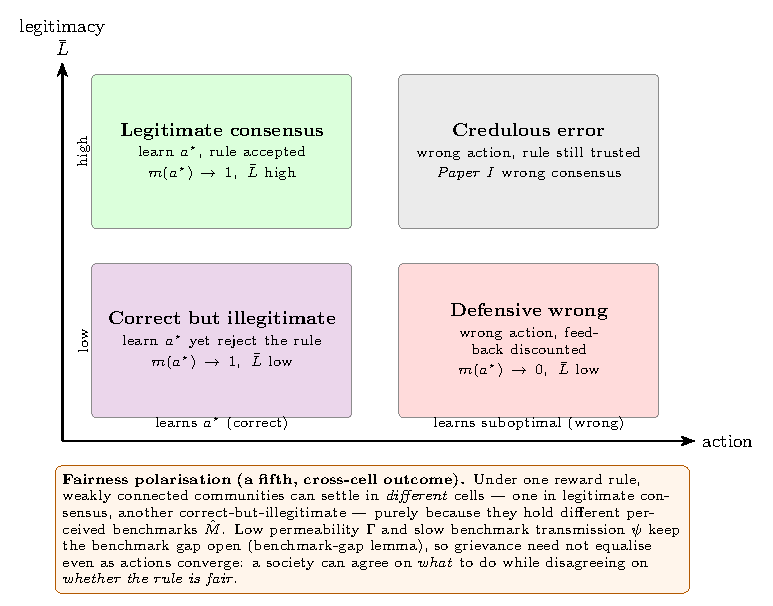
\includegraphics[width=0.82\textwidth]{fig_regimemap.pdf}
\caption{Regime map. The two collective achievements --- learning the optimal
action and accepting the rule as legitimate --- are independent axes. Legitimate
consensus and defensive wrong consensus lie on one diagonal; correct-but-
illegitimate consensus and credulous error (the wrong consensus of the
credibility baseline) on the other. Fairness polarisation is communities
occupying different cells under the same rule.}
\label{fig:regimemap}
\end{figure}

\section{Simulation design}
\label{sec:design}

\paragraph{Information structure.}
Before choosing, agents observe neighbours' previous actions and confidence
signals (the credibility field). After outcomes are realised, they observe
neighbours' actions, realised rewards and confidence for the retrospective
channel, and they observe their own realised reward relative to the perceived
modal-agent benchmark. Confidence is communicated or behaviourally inferred
subjective reliability, not objective accuracy; the modal-agent benchmark is a
perceived entitlement, not the true rule.

We use two communities, binary actions, stationary rewards, balanced block
weights, and a synchronous simultaneous update. Observables include
community action mass $m_{c,t}(a)$, mean legitimacy $\bar L_{c,t}$, the perceived
benchmark $\bar{\hat M}_{c,t}$, the acceptability rate, the evidence-discount gap
$|\delta|-|\delta^{\mathrm{eff}}|$, the legitimacy gap $G^L_t=|\bar L_{1,t}-\bar
L_{2,t}|$, and the modal-agent gap $G^M_t$. Terminal outcomes are classified as
\emph{legitimate consensus} (both communities place $\ge\theta$ on $a^\star$ and
mean legitimacy is high), \emph{correct-but-illegitimate} (optimal-arm consensus,
low legitimacy), \emph{defensive wrong} (suboptimal-arm consensus, low
legitimacy), \emph{fairness polarisation} (communities differ in legitimacy or
action), or unresolved. Regime probabilities are Monte Carlo frequencies; the
implementation passes the verification suite of Appendix~\ref{app:tests} before
any experiment is run. Default and per-experiment parameters are in
Appendix~\ref{app:params}; the replication package is authoritative.
Table~\ref{tab:comparison} positions the model and Table~\ref{tab:variables}
lists the variables.

\paragraph{Uncertainty reporting.} Regime probabilities are empirical frequencies
over independent replications, reported with Wilson 95\% intervals; means carry
Monte Carlo standard errors and percentile-bootstrap 95\% intervals. The ablations
(Section~\ref{sec:results-ablation}) use common random numbers --- the same seed,
hence the same exogenous reward and decision-noise environment, across variants,
with realised rewards following each variant's action path --- so the
full-vs-ablation paired difference identifies a component's effect, reported with
a paired-bootstrap 95\% interval.

\begin{table}[t]\centering\small
\caption{Positioning relative to adjacent model families.}
\label{tab:comparison}
\begin{tabular}{p{3.0cm}p{3.3cm}p{2.7cm}p{3.4cm}}\toprule
Tradition & Typical mechanism & Feedback authority & What this paper changes \\ \midrule
Social/RL learning & reward-driven value update & fixed (always valid) & legitimacy gate on evidence \\
Inequity aversion & reference-dependent utility & one-shot, no learning & fairness inside a learning loop \\
Legitimacy / proc.\ justice & rule acceptance & exogenous & endogenous, socially learned \\
Opinion dynamics & weighted averaging & no reward rule & reward legitimacy as state \\
Credibility (Paper~I) & confidence-weighted transmission & valid evidence & feedback can be delegitimised \\
\bottomrule\end{tabular}
\end{table}

\begin{table}[t]\centering\small
\caption{Model variables and interpretations.}
\label{tab:variables}
\begin{tabular}{ll}\toprule Symbol & Interpretation \\ \midrule
$Q_{i,t}(a)$ & latent action value \\
$C_{i,t}$ & endogenous confidence (balance of evidence) \\
$S_{i,t}(a)$ & credibility-weighted social signal \\
$L_{i,t}$ & legitimacy of the reward rule (gates evidence) \\
$\hat M_{i,t}$ & perceived modal-agent fairness benchmark \\
$M$ & true modal-agent benchmark \\
$\Delta^F_{i,t}$ & fairness discrepancy $R-r^F$ \\
$D^F_{i,t}$ & asymmetric fairness discomfort \\
$\delta^{\mathrm{eff}}_{i,t}$ & legitimacy-gated prediction error $L\,\delta$ \\
\bottomrule\end{tabular}
\end{table}


\section{Results}
\label{sec:results}

\paragraph{II.1 Agents mind unfairness more when it harms them.}
Holding the absolute fairness deviation fixed, disadvantageous unfairness
($\Delta^F<0$) erodes legitimacy far more than advantageous unfairness
($\Delta^F>0$), because $\phi^->\phi^+$ pushes disadvantageous discomfort across
the acceptability threshold while advantageous discomfort stays below it
(Figure~\ref{fig:asym}). This asymmetry is the engine of the regimes below:
under-reward is delegitimising, over-reward is tolerated.

\begin{figure}[t]
\centering
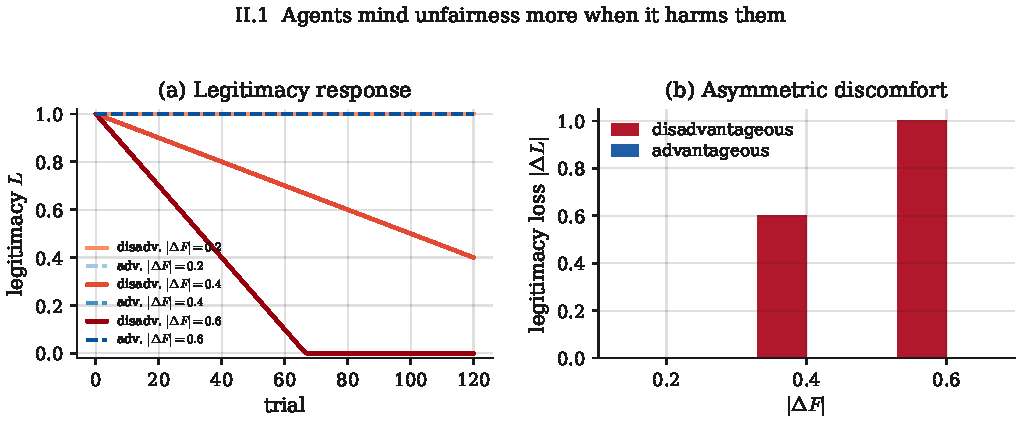
\includegraphics[width=\textwidth]{fig2_asymmetry.pdf}
\caption{II.1. (a) Legitimacy trajectories under a fixed fairness deviation, by
sign and magnitude. (b) Legitimacy loss is large for disadvantageous and
negligible for advantageous unfairness.}
\label{fig:asym}
\end{figure}

\paragraph{II.2 An acceptability threshold separates tolerance from collapse.}
Sweeping $\tau^F$ at a fixed level of unfairness, terminal mean legitimacy rises
from near $0$ to near $1$ (Figure~\ref{fig:fair}c): a low threshold makes
unfairness delegitimising, a high threshold makes it tolerable, with a steep
transition between. This is the empirical counterpart of
Proposition~\ref{prop:drift}.

\paragraph{II.3 Fairness polarisation without payoff differences.}
Two communities under the \emph{same} reward rule, but with opposed modal-agent
benchmarks ($\hat M_1=0.25$, $\hat M_2=0.75$) and low permeability, polarise in
legitimacy: the low-entitlement community keeps $\bar L\approx 1$ while the
high-entitlement community falls to $\bar L\approx 0.37$, a terminal gap
$G^L\approx 0.63$ (Figure~\ref{fig:fair}a,b). Because benchmarks transmit slowly
under low permeability, the difference persists. Identical material payoffs thus
produce divergent legitimacy purely through divergent fairness benchmarks.

\begin{figure}[t]
\centering
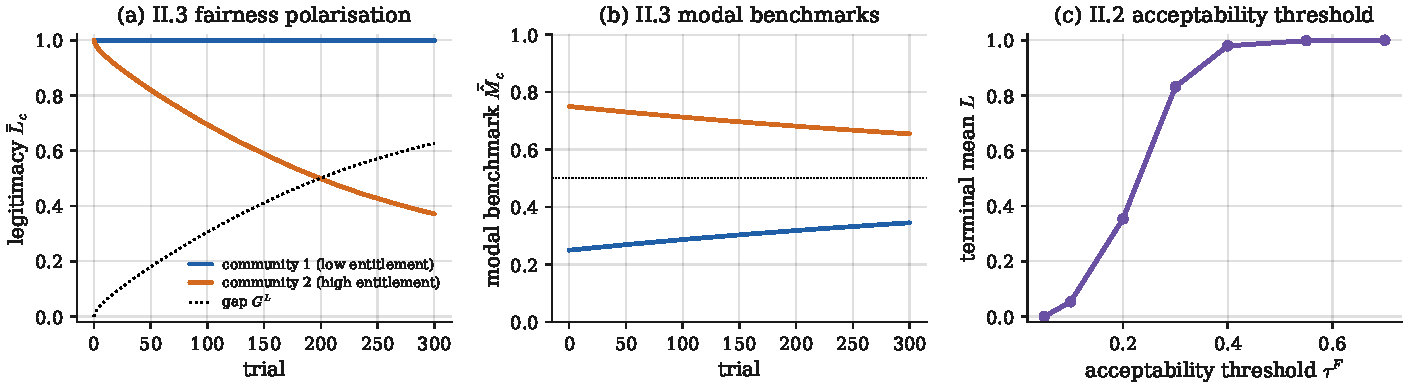
\includegraphics[width=\textwidth]{fig3_fairness.pdf}
\caption{(a) II.3 community legitimacy and the gap $G^L$; (b) II.3 modal-agent
benchmarks remain split under low permeability; (c) II.2 terminal mean legitimacy
versus the acceptability threshold $\tau^F$.}
\label{fig:fair}
\end{figure}

\paragraph{II.4 Legitimacy gating makes wrong consensus persistent.}
This is the central result (Figure~\ref{fig:regimes}a). At a moderate
transmission strength with an early lead on the suboptimal arm, the \emph{ungated}
model self-corrects: terminal optimal-arm mass $m(a^\star)=0.93$ (legitimate
consensus). Switching on the legitimacy gate, with the benchmark set so that the
poorly paying arm feels unfair, legitimacy collapses while agents are still on the
wrong arm; corrective feedback then loses authority ($\delta^{\mathrm{eff}}=L\delta\to0$),
and the same configuration locks onto the wrong action: $m(a^\star)=0.01$, $\bar
L=0.01$ --- defensive wrong consensus. Adding modal-agent misrepresentation leaves
the outcome wrong and lowers legitimacy further. Negative evidence loses its
disciplining power exactly when it is most needed.

\begin{figure}[t]
\centering
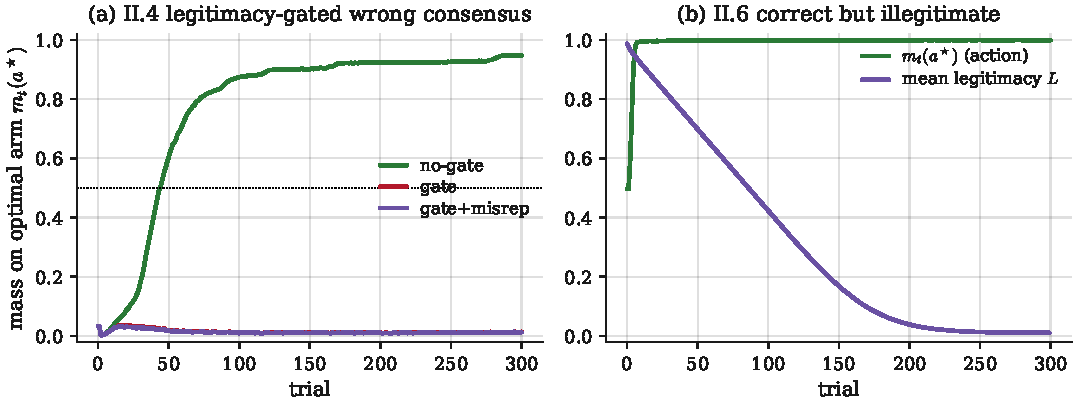
\includegraphics[width=\textwidth]{fig4_regimes.pdf}
\caption{(a) II.4: with the legitimacy gate off the society corrects an early
wrong lead ($m(a^\star)\to0.93$); with the gate on it locks onto the wrong arm
($\to0.01$). (b) II.6: agents learn the optimal action ($m(a^\star)\to1$) while
mean legitimacy decays to near zero --- correct but illegitimate.}
\label{fig:regimes}
\end{figure}

\paragraph{II.5 Network geometry tunes legitimacy and its polarisation.}
Varying cross-community permeability $\Gamma$ on the misrepresentation setup,
low permeability sustains a large legitimacy gap $G^L$ (fairness polarisation)
while high permeability mixes benchmarks toward a common value and a common
legitimacy level (Figure~\ref{fig:geom}). Permeability that would spread
corrective information in a pure credibility model here also spreads fairness
benchmarks, so its effect on collective legitimacy is not monotone in welfare.

\begin{figure}[t]
\centering
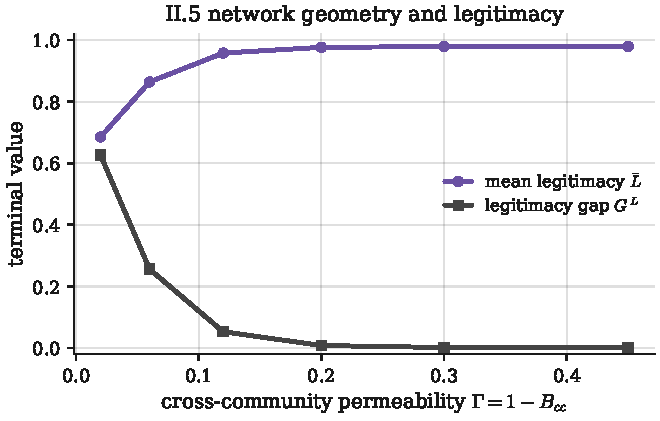
\includegraphics[width=0.62\textwidth]{fig5_geometry.pdf}
\caption{II.5. Terminal mean legitimacy $\bar L$ and the legitimacy gap $G^L$
versus permeability $\Gamma$.}
\label{fig:geom}
\end{figure}

\paragraph{II.6 Epistemic success and legitimacy failure can diverge.}
When the optimal arm is learnable but the entitlement benchmark is high, agents
learn what works yet stop believing the rule is fair: $m(a^\star)\to1$ while mean
legitimacy decays to $\approx0.01$ (Figure~\ref{fig:regimes}b). Correct beliefs
and accepted rules are distinct collective achievements.

\subsection{Phase diagrams}
\label{sec:results-phase}
Figure~\ref{fig:phase} maps the regimes. The \emph{main} phase diagram sweeps the
acceptability threshold $\tau^F$ against the initial benchmark disagreement
$|\Delta\hat M_0|$ (with a learnable optimum, so action consensus forms and
defensive-wrong does not arise in this slice). Three regimes tile the plane: a
high-$\tau^F$ band of legitimate consensus; a low-$\tau^F$ band of
correct-but-illegitimate consensus (both communities delegitimise); and a
fairness-polarisation wedge at intermediate $\tau^F$ with large benchmark
disagreement, where the high-entitlement community delegitimises while the
low-entitlement one does not. The \emph{secondary} diagram shows that the
legitimacy gap $G^L$ is large only when permeability $\Gamma$ \emph{and} modal
transmission $\psi$ are both small: fairness polarisation requires that distorted
benchmarks neither mix across communities nor average within them. Geometry that
spreads information also dissolves grievance.

\begin{figure}[t]
\centering
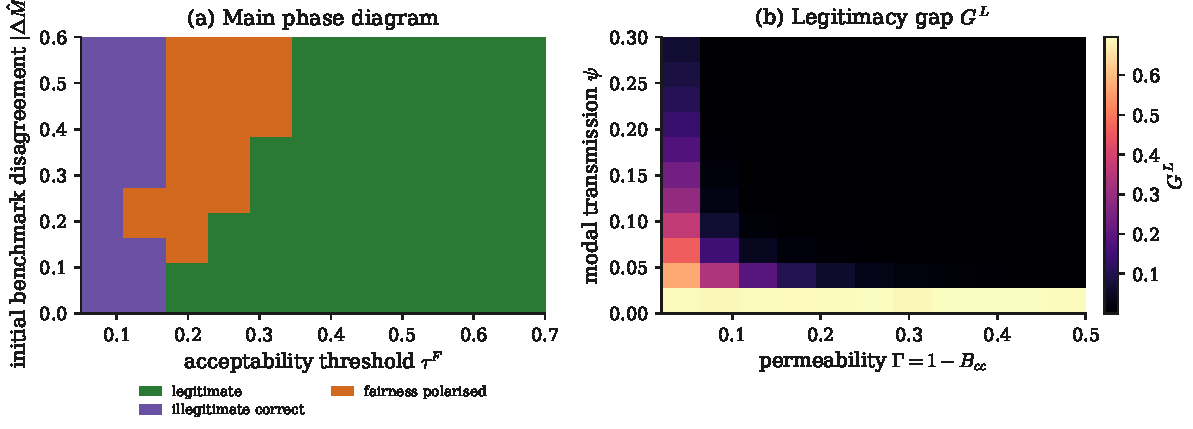
\includegraphics[width=\textwidth]{fig6_phase.pdf}
\caption{Phase diagrams ($R=60$ per cell, $11\times11$). (a) terminal regime over
$\tau^F$ (acceptability) and $|\Delta\hat M_0|$ (initial benchmark disagreement).
(b) legitimacy gap $G^L$ over permeability $\Gamma$ and modal transmission $\psi$.}
\label{fig:phase}
\end{figure}

\subsection{Which components are necessary? Ablations}
\label{sec:results-ablation}
At the legitimacy-gated wrong-consensus operating point ($R=200$, common random
numbers), the full model produces defensive wrong consensus with probability
$1.00$. Figure~\ref{fig:ablations} and Table~\ref{tab:ablation} report the paired
counterfactual effects. Two components are \emph{necessary}: removing the
legitimacy gate (A1) restores correction ($m(a^\star)\!:0.01\!\to\!0.91$,
$\Delta=+0.93$), and removing the credibility field (A6) prevents the wrong
\emph{action} from locking in ($m(a^\star)\to0.79$) although legitimacy still
collapses ($\bar L\to0.01$) --- the gate alone yields correct-but-illegitimate,
not defensive-wrong. The retrospective channel (A7) is \emph{contributory}
($\Delta=+0.15$). Modal-agent misrepresentation and the discomfort asymmetry
(A2--A5) are \emph{not} necessary for defensive wrong consensus at this point ---
they instead drive the fairness-polarisation regime. Defensive wrong consensus is
thus the conjunction of legitimacy collapse (the gate) and credibility-weighted
amplification (the field).

\begin{figure}[t]
\centering
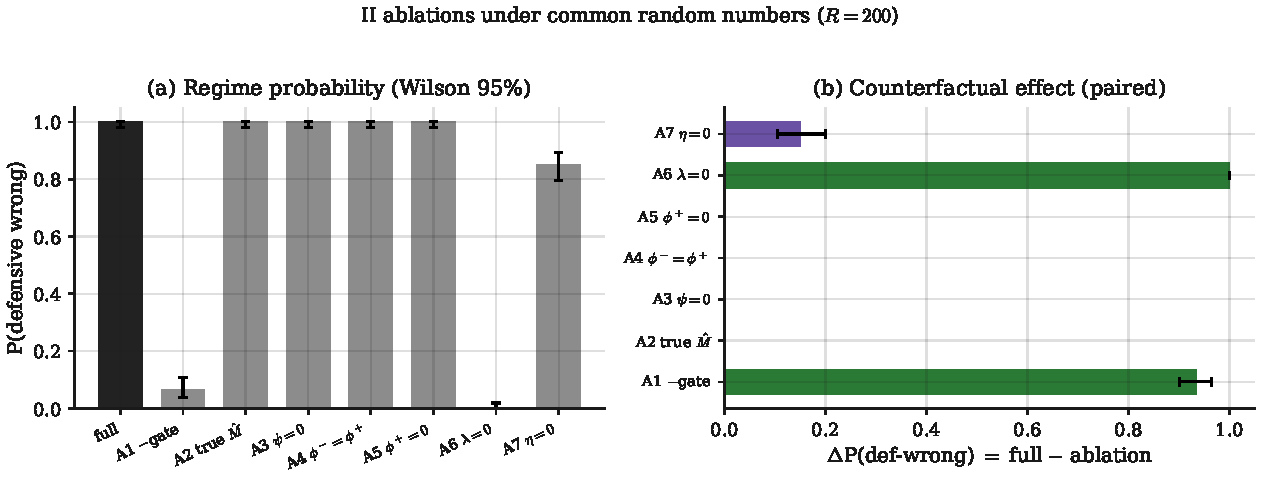
\includegraphics[width=\textwidth]{fig7_ablations.pdf}
\caption{Ablations under common random numbers ($R=200$). (a) P(defensive wrong)
per variant with Wilson 95\% intervals; (b) paired counterfactual effect
$\Delta=$P(def.-wrong$\mid$full)$-$P(def.-wrong$\mid$ablation) with paired-bootstrap
95\% intervals. Green: necessary; purple: contributory; grey: not necessary.}
\label{fig:ablations}
\end{figure}

% Auto-generated -- experiment outcomes.
\begin{table}[t]\centering\small
\caption{Experiment outcomes (standard scale). $m(a^\star)$ is terminal optimal-arm mass; $\bar L$ is terminal mean legitimacy; $G^L$ is the between-community legitimacy gap. Scenario parameters: \texttt{code/legitimacy/scenarios.py}.}
\label{tab:results}
\begin{tabular}{lll}\toprule
Experiment & Manipulation & Outcome \\ \midrule
II.1 adv.\ vs disadv. & $\Delta^F=\pm x$, $|x|$ fixed & legitimacy loss 1.00 (disadv.) vs 0.00 (adv.) \\
II.2 acceptability & sweep $\tau^F$ & mean $L$ rises $0.05\!\to\!1.00$ across $\tau^F$ \\
II.3 modal misrep. & $\hat M_1\neq\hat M_2$ & fairness polarisation, $G^L=0.63$ \\
II.4 no gate & legitimacy off & $m(a^\star)=0.93$, legitimate consensus \\
\quad\ gate & legitimacy on & $m(a^\star)=0.01$, $\bar L=0.01$: \textbf{defensive wrong} \\
II.6 correct/illegit. & high entitlement & $m(a^\star)=1.00$, $\bar L=0.01$ \\
\bottomrule\end{tabular}
\end{table}

% Auto-generated -- ablations.
\begin{table}[t]\centering\small
\caption{Ablation effects at the legitimacy-gated wrong-consensus operating point, $R=200$ under common random numbers. P(def.-wrong) carries a Wilson 95\% interval; $\Delta$ is the paired counterfactual effect full$-$ablation with a paired-bootstrap 95\% interval.}
\label{tab:ablation}
\begin{tabular}{lccc}\toprule
Variant & P(def.-wrong) [95\%] & $m(a^\star)$ & $\Delta$P(def.-wrong) [95\%] \\ \midrule
full & 1.00 [0.98, 1.00] & 0.01 & --- \\
A1 no gate & 0.07 [0.04, 0.11] & 0.91 & $+0.94$ [+0.90, +0.96] \\
A2 true $\hat M$ & 1.00 [0.98, 1.00] & 0.01 & $+0.00$ [+0.00, +0.00] \\
A3 $\psi{=}0$ & 1.00 [0.98, 1.00] & 0.01 & $+0.00$ [+0.00, +0.00] \\
A4 $\phi^-{=}\phi^+$ & 1.00 [0.98, 1.00] & 0.01 & $+0.00$ [+0.00, +0.00] \\
A5 $\phi^+{=}0$ & 1.00 [0.98, 1.00] & 0.01 & $+0.00$ [+0.00, +0.00] \\
A6 $\lambda{=}0$ & 0.00 [0.00, 0.02] & 0.79 & $+1.00$ [+1.00, +1.00] \\
A7 $\eta{=}0$ & 0.85 [0.79, 0.89] & 0.17 & $+0.15$ [+0.10, +0.20] \\
\bottomrule\end{tabular}
\end{table}


\section{Equilibrium interpretation}
\label{sec:equilibrium}
The model is a dynamic learning process, not an equilibrium solved each period,
but its absorbing regimes have clean readings in behavioural game theory.

\emph{A mean-field phase portrait.} The model admits a deterministic
large-population reduction (\texttt{legitimacy/meanfield.py}): with a scalar
benchmark $\hat M$ held fixed, the state collapses to the value contrast
$\Delta=Q(a^\star)-Q(\text{other})$ and the shared legitimacy $L$, with choices
following the exact quantal (logistic) map and rewards, the gated update and the
legitimacy update taken in expectation. Motivated cognition makes legitimacy a
\emph{self-reinforcing attitude} rather than a passively eroding quantity: a
legitimate stance disposes agents to read outcomes charitably, an illegitimate
one to read them as further grievance \citep{Kunda1990,Festinger1957}. We encode
this as a tilted double well (cusp) for $x=L-\tfrac12$,
\begin{equation}
\dot x = r\,x - s\,x^3 + h(\hat M),\qquad
h(\hat M)=-\mu_{\mathrm{t}}\big(\bar D^F(\hat M)-\tau^F\big),
\label{eq:cusp}
\end{equation}
where the tilt $h$ decreases in perceived unfairness $\bar D^F-\tau^F$ and $r>0$
is the strength of the self-reinforcement. The constants are \emph{calibrated
from the model} (\texttt{calibrate\_cusp}): the tilt vanishes at the
discomfort-balance benchmark $\hat M^\star$ (where $\bar D^F=\tau^F$); the two
wells are pinned to the model's birth-death legitimacy levels
$\nu_R a/(\nu_R a+\nu_F e)$ --- with acceptance rate $a$ and expected excess
discomfort $e$ from the fairness rates $\nu_R,\nu_F,\phi^\pm,\tau^F$ --- evaluated
at the fair and unfair edges of the fold band; the tilt gain then places the two
folds symmetrically about $\hat M^\star$. Only the self-reinforcement strength has
no baseline counterpart. Its rest points are the
(choice, legitimacy) equilibria; the flow is the phase portrait of
Figure~\ref{fig:phaseportrait}. Because $\Delta$ relaxes toward the correct
contrast whenever $L>0$, the value coordinate is monostable, but legitimacy is
bistable: for a \emph{fair} rule the plane has one interior attractor at high
legitimacy (legitimate consensus), for an \emph{unfair} rule one interior
attractor at low legitimacy (correct-but-illegitimate), and for
\emph{intermediate} entitlement \emph{two} interior attractors separated by a
saddle. Sweeping $\hat M$ therefore traces a fold with hysteresis
(Figure~\ref{fig:eqm}a): two stable legitimacy branches joined by an unstable
one, colliding at two folds, so history --- not payoffs --- selects which regime a
community occupies. Legitimacy does not change the quantal response itself; it
decides where on it the state settles (Figure~\ref{fig:eqm}b). The additive,
hard-clipped rule of Section~\ref{sec:model} is the singular limit of
\eqref{eq:cusp} in which the wells are pushed to the boundaries $L\in\{0,1\}$;
defensive-wrong consensus is then the $L\!\to\!0$ frozen corner.

\begin{figure}[t]
\centering
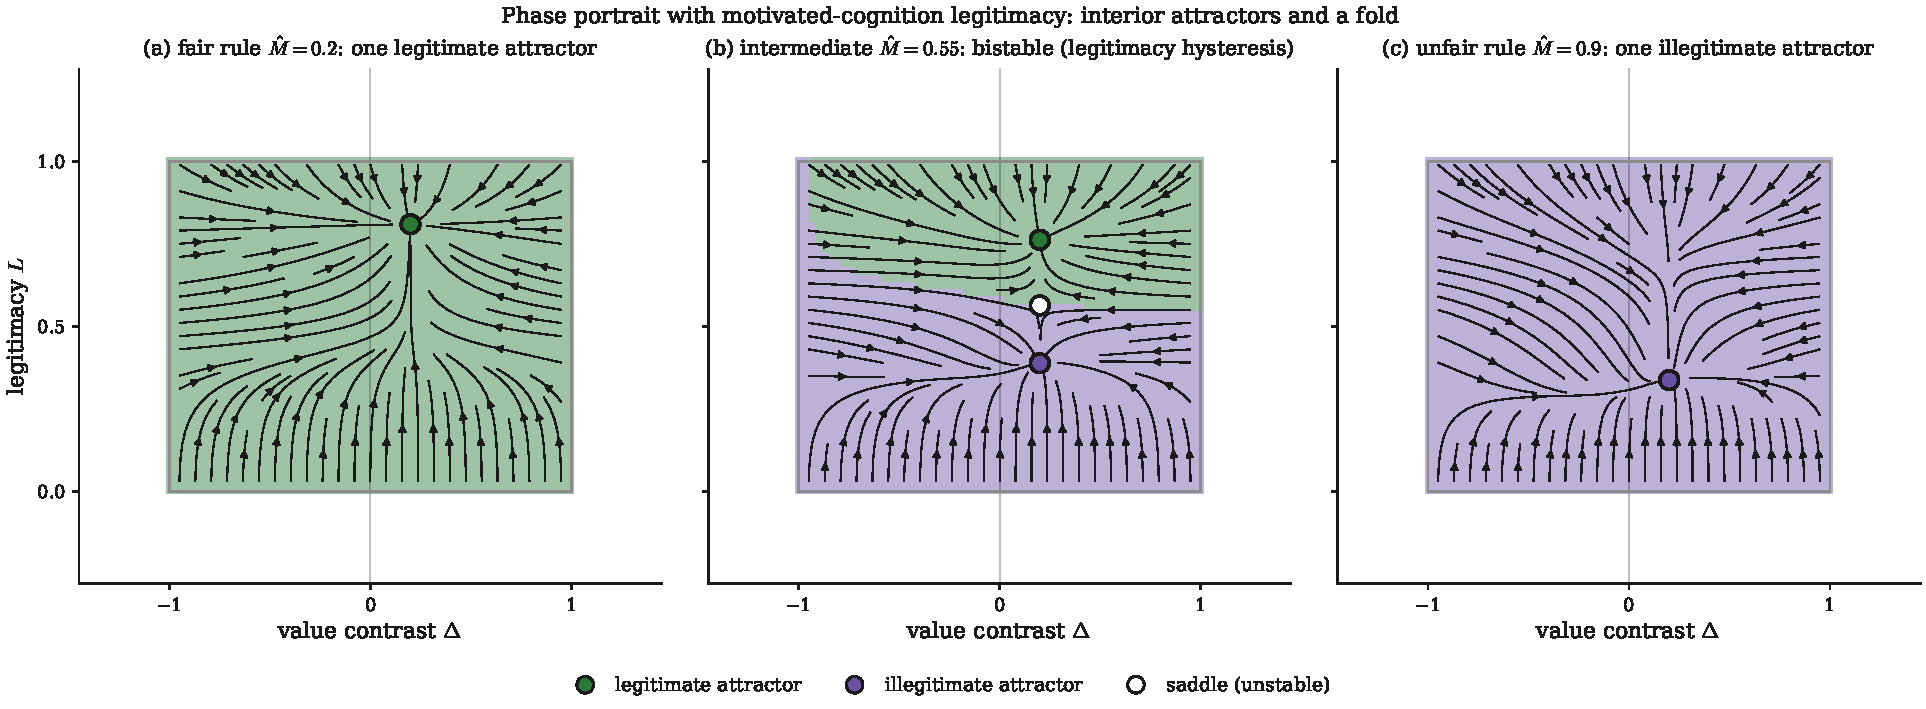
\includegraphics[width=\textwidth]{fig8_phase_portrait.pdf}
\caption{Phase portrait of the mean-field reduction with motivated-cognition
legitimacy \eqref{eq:cusp}, streamlines over basins of attraction; filled markers
are stable attractors, open markers saddles. \textbf{(a)}~Fair rule ($\hat M=0.2$):
a single interior attractor at high legitimacy. \textbf{(b)}~Intermediate
($\hat M=0.55$): \emph{bistable} --- a legitimate and an illegitimate interior
attractor separated by a saddle (legitimacy hysteresis). \textbf{(c)}~Unfair rule
($\hat M=0.9$): a single interior attractor at low legitimacy. The value contrast
corrects in every case ($L>0$); the communities differ in \emph{legitimacy}, not
in action.}
\label{fig:phaseportrait}
\end{figure}

\begin{figure}[t]
\centering
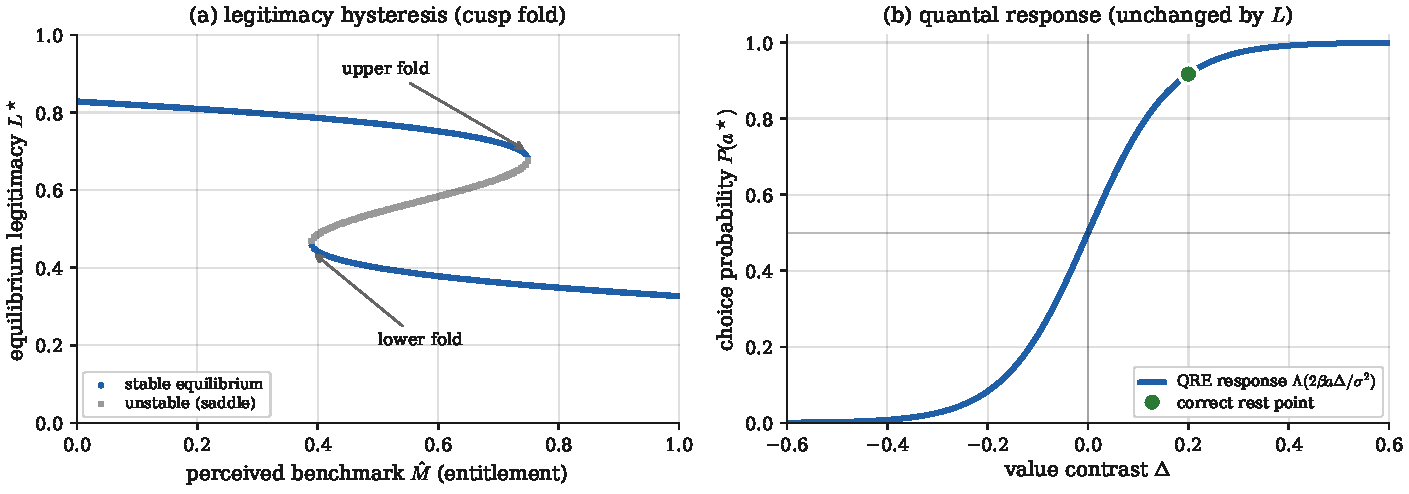
\includegraphics[width=0.92\textwidth]{fig9_equilibrium.pdf}
\caption{\textbf{(a)}~Legitimacy hysteresis: the equilibrium legitimacy $L^\star$
versus perceived benchmark $\hat M$ is an S-curve --- two stable branches
(high/low legitimacy) joined by an unstable saddle branch, meeting at two folds
(a cusp catastrophe). Between the folds the outcome is history-dependent.
\textbf{(b)}~The quantal-response choice map is unchanged by legitimacy; the gate
decides where on it the state settles.}
\label{fig:eqm}
\end{figure}

\emph{Quantal response.} The logistic choice rule is a quantal best response to
the augmented value contrast, so a consensus rest point --- at which a community's
action frequencies reproduce themselves under the choice map --- is a
quantal-response fixed point in the sense of \citet{McKelveyPalfrey1995}. The
regimes are thus stable rest points of a quantal-response dynamic, and legitimacy
gating changes which rest point is reached by reweighting the evidence that moves
values.

\emph{Fairness preferences.} The legitimacy channel embeds reference-dependent,
asymmetric fairness relative to a benchmark, the same primitive as inequity
aversion and reciprocity models \citep{Rabin1993Fairness,FehrSchmidt1999,BoltonOckenfels2000};
a low-legitimacy rest point is one at which agents' fairness evaluations against
the modal benchmark are self-sustaining.

\emph{Set-valued (M) equilibrium.} That the \emph{same} reward rule supports
several regimes --- legitimate, correct-but-illegitimate, and fairness-polarised
(Figure~\ref{fig:phase}) --- is naturally read as a set-valued solution. In the
M-equilibrium of \citet{GoereeLouis2021}, choices are monotone and beliefs are
consequentially unbiased; the fairness-polarisation regime is exactly the case in
which community beliefs about the modal agent are \emph{not} consequentially
unbiased, so distinct self-consistent (choice, belief) sets coexist.

\emph{Bounded reasoning about a modal agent.} The perceived benchmark $\hat
M_{i,t}$ is a belief about a representative other to which agents best respond
through fairness discomfort --- a level-$1$ / cognitive-hierarchy construct
\citep{Nagel1995,StahlWilson1995,CamererHoChong2004}. Misrepresentation is
precisely heterogeneous, incorrect beliefs about that modal agent, and
Eq.~\eqref{eq:Mupdate} is a social process by which such beliefs do or do not
converge.

\emph{Evolutionary stability.} The corner attractors of the phase portrait are
locally stable: a small perturbation of choices or legitimacy decays back
(Figure~\ref{fig:phaseportrait}). Each is therefore convention-like --- an
evolutionarily stable rest point of the population dynamic that resists small
invasions. The defensive-wrong consensus is the cautionary case: it is a stable
convention built on a mis-calibrated benchmark, so once a community has entered
its basin, restoring accurate feedback does not dislodge it --- the feedback is no
longer admitted as evidence.

\begin{proposition}[Rest points and their equilibrium reading]
\label{prop:equilibrium}
Consider the deterministic community recursion. (i) A symmetric consensus rest
point is a quantal-response fixed point of the augmented-value game. (ii) If
communities begin with disagreeing benchmarks and permeability and modal
transmission are small, the recursion admits distinct community-level rest points
(a polarised configuration); reading action frequencies as choices and perceived
benchmarks as beliefs, this is an M-equilibrium whose beliefs are not
consequentially unbiased across communities.
\end{proposition}
\noindent (Proof in Appendix~\ref{app:proofs}.)

\subsection{A complete characterisation of the behavioural equilibrium}
\label{sec:characterisation}
Write the mean-field map of Section~\ref{sec:equilibrium} as an operator
$T_{\hat M}$ on the community state $(Q,L)\in[0,1]^2\times[0,1]$: choices are the
quantal response to the augmented value, and rewards, the legitimacy-gated value
update and the expected legitimacy update are taken in expectation. A
\emph{behavioural equilibrium} at benchmark $\hat M$ is a fixed point
$T_{\hat M}(Q^\star,L^\star)=(Q^\star,L^\star)$: a self-consistent
(choice distribution, values, legitimacy) triple reproduced by gated learning and
quantal choice.

\begin{proposition}[Existence and value nullcline]
\label{prop:existence}
For every $\hat M$, $T_{\hat M}$ is continuous on a compact convex set, so a
behavioural equilibrium exists (Brouwer). At any equilibrium with $L^\star>0$ the
gated value nullcline forces $Q^\star(a)=\mu_a$ on both arms, so the contrast is
$\Delta^\star=\mu_{a^\star}-\mu_o>0$ and the choice is the quantal response
$\Lambda(2\beta a\Delta^\star/\sigma^2)$; only at $L^\star=0$ can $Q^\star$ be
frozen away from the reward means. The value coordinate is therefore monostable
whenever legitimacy is positive, and the equilibrium set is indexed by the
legitimacy roots of the cusp \eqref{eq:cusp}.
\end{proposition}

\begin{proposition}[Legitimacy bistability, folds, and hysteresis]
\label{prop:hysteresis}
Write $x=L-\tfrac12$ and the tilt $h(\hat M)=-\mu_{\mathrm t}(\bar D^F(\hat M)-\tau^F)$,
increasing in perceived unfairness. The interior legitimacy equilibria are the
roots of $x^3-(r/s)x-h/s=0$. For $|h|<h_c:=2s\,(r/(3s))^{3/2}$ there are
\emph{three} equilibria --- two stable (a legitimate $L^\star_+$ and an
illegitimate $L^\star_-$, both interior) separated by an unstable saddle --- and
for $|h|>h_c$ a single stable equilibrium. As $\hat M$ increases through the band
where $|h(\hat M)|<h_c$, the system traverses a bistable region bounded by two
saddle-node (fold) bifurcations at $h=\pm h_c$: legitimacy is \emph{hysteretic}
(a cusp catastrophe), and within the band the attained regime is selected by
history, not by $\hat M$ (Figure~\ref{fig:eqm}a). A stable equilibrium at
$x^\star$ is asymptotically stable because $r-3s\,x^{\star2}<0$ there.
\end{proposition}

\noindent Under community heterogeneity the picture is additionally set-valued:
Proposition~\ref{prop:equilibrium} and Lemma~\ref{lem:gap} give that when
$\psi\Gamma$ is small the benchmark gap persists and distinct community-level
equilibria coexist --- an M-equilibrium whose beliefs are not consequentially
unbiased across communities \citep{GoereeLouis2021}, reducing to a regular quantal
response equilibrium \citep{McKelveyPalfrey1995} in the symmetric,
single-benchmark case. The additive, hard-clipped legitimacy rule of
Section~\ref{sec:model} is the singular limit in which the two wells sit at the
boundaries $L\in\{0,1\}$ and the fold degenerates to a boundary transcritical at
$\hat M^\star=(\tau^F+\nu_R\mu_{a^\star}/[\nu_F(1-\mu_{a^\star})])/\phi^-$;
defensive-wrong consensus is then the frozen $L\!\to\!0$ corner. Proofs of
Propositions~\ref{prop:existence} and~\ref{prop:hysteresis} are in
Appendix~\ref{app:proofs}.

\paragraph{Dynamic-programming formulation.}
Each agent's value estimate follows the legitimacy-gated Robbins--Monro recursion
$Q_{t+1}(a)=Q_t(a)+\alpha L\,(R-Q_t(a))$ on visits, whose decreasing-step limit is
the stochastic-approximation ODE $\dot Q(a)=L\,(\E[R\mid a]-Q(a))$
\citep{Borkar2008}. The associated gated Bellman/TD operator
$\mathcal T_L Q(a)=Q(a)+L\,(\E[R\mid a]-Q(a))$ is a contraction of modulus
$1-\alpha L$ with unique fixed point $Q^\star(a)=\E[R\mid a]$ when $L>0$, and the
identity map (learning halts) at $L=0$. Legitimacy is thus a state-dependent
weight on the reward-prediction-error backup --- a reference-dependent Markov
decision process whose effective reward signal is $L\,\delta$, the population-level
analogue of a gated prediction-error readout
\citep{JoinerPivaTurrinChang2017}. The interaction is a mean-field (population)
game: each agent's gated MDP is coupled to the others through the anticipatory
field $S$ and the transmitted benchmark $\hat M$, and a behavioural equilibrium is
the consistency point of quantal best response with gated learning --- a
mean-field game with a legitimacy-gated Bellman operator, whose equilibrium
selection is governed by Proposition~\ref{prop:hysteresis}.

\section{Discussion}
\label{sec:discussion}
Three claims follow. First, the authority of feedback is a state variable, not a
constant: once legitimacy is endogenous, the same reward stream can teach a lot or
nothing, and collective error can be defended rather than corrected. Second,
fairness benchmarks are social: because the modal-agent benchmark is transmitted
on the network, communities can polarise in legitimacy under identical payoffs,
and network geometry that spreads information also spreads grievance. Third,
epistemic and legitimacy outcomes are independent axes: a society can be right and
aggrieved (correct-but-illegitimate) or wrong and self-justifying (defensive
wrong). Relative to the credibility baseline \citep{BontempsBanerjee2026}, the new
and policy-relevant failure mode is that interventions which restore accurate
feedback may not help if that feedback is no longer treated as legitimate.

\paragraph{Cognitive interpretation of the parameters.}
The parameters carry direct psychological readings. The asymmetric discomfort
weights $\phi^->\phi^+$ encode loss-averse, self-serving fairness: shortfalls
below the benchmark hurt more than windfalls please, the reference-dependent form
of inequity aversion \citep{FehrSchmidt1999} placed inside a learning loop. The
acceptability threshold $\tau^F$ is a tolerance for perceived unfairness before
legitimacy erodes; the loss and recovery rates $\nu_F,\nu_R$ are the speed of
delegitimation and of its repair; the benchmark transmission rate $\psi$ is
susceptibility to socially communicated grievance; and the perceived benchmark
$\hat M$ is a (possibly distorted) belief about what a representative agent is
entitled to. Legitimacy $L$ itself is the evidential weight the agent grants to
reward feedback --- a motivated-cognition gain on the prediction error rather
than on the choice.

\paragraph{A normative benchmark.}
The natural reference is the \emph{ungated} learner ($L\equiv1$), for which reward
feedback retains full authority --- the epistemic ideal in which evidence always
teaches. At the collapse operating point the gate is costly in exactly this
sense: removing it (ablation A1) lifts the population mass on the optimal action
from $m(a^\star)\approx0.01$ to $0.91$ and cuts defensive-wrong consensus from
$P=1.00$ to $0.07$ (Table~\ref{tab:ablation}). Legitimacy gating is therefore not
epistemically neutral: at this point it converts a nearly-correct society into a
nearly-certainly-wrong one, a $\sim\!90$ percentage-point loss of correct-action
adoption that measures the welfare cost of illegitimacy. The same gate is
protective elsewhere (it lets a community withhold assent from a genuinely unfair
rule); the model makes the trade-off explicit rather than assuming feedback is
always admitted.

\paragraph{Testable predictions.}
The mechanism yields lab-testable predictions. \textbf{(i)} Manipulating perceived
fairness \emph{without} changing payoffs --- by shifting the communicated
modal-agent benchmark --- should change how much people learn from identical
reward feedback, measurable as a slower value update (smaller learning rate) under
low perceived legitimacy. \textbf{(ii)} The loss/gain asymmetry $\phi^->\phi^+$
predicts that below-benchmark outcomes erode legitimacy faster than equal
above-benchmark outcomes restore it, an asymmetry recoverable from trial-by-trial
legitimacy or acceptance ratings. \textbf{(iii)} An acceptability threshold
predicts a nonlinear, hysteretic collapse: legitimacy is stable under small
unfairness and drops sharply once discrepancy exceeds $\tau^F$. \textbf{(iv)}
Because benchmarks are transmitted, seeding two weakly connected groups with
different fairness benchmarks should produce divergent legitimacy --- and even
divergent choices --- under identical payoffs, with the divergence controlled by
inter-group permeability. \textbf{(v)} Legitimacy and its benchmark are
\emph{latent}: estimate them per trial from acceptance ratings, response times and
fairness reports, and test whether the gated-update model (learning rate scaling
with inferred legitimacy) predicts behaviour better than an ungated learner.
\textbf{(vi)} Because the defensive-wrong state is a stable attractor
(Figure~\ref{fig:phaseportrait}b), restoring accurate feedback to a group already
in its basin should \emph{not} correct it, whereas restoring legitimacy ---
reducing perceived unfairness --- should reopen learning: a testable dissociation
between ``better information'' and ``fairer rule'' interventions. Each maps onto a
manipulable quantity in reward-learning or public-goods paradigms with a fairness
manipulation (Figure~\ref{fig:experiment}).

\begin{figure}[t]
\centering
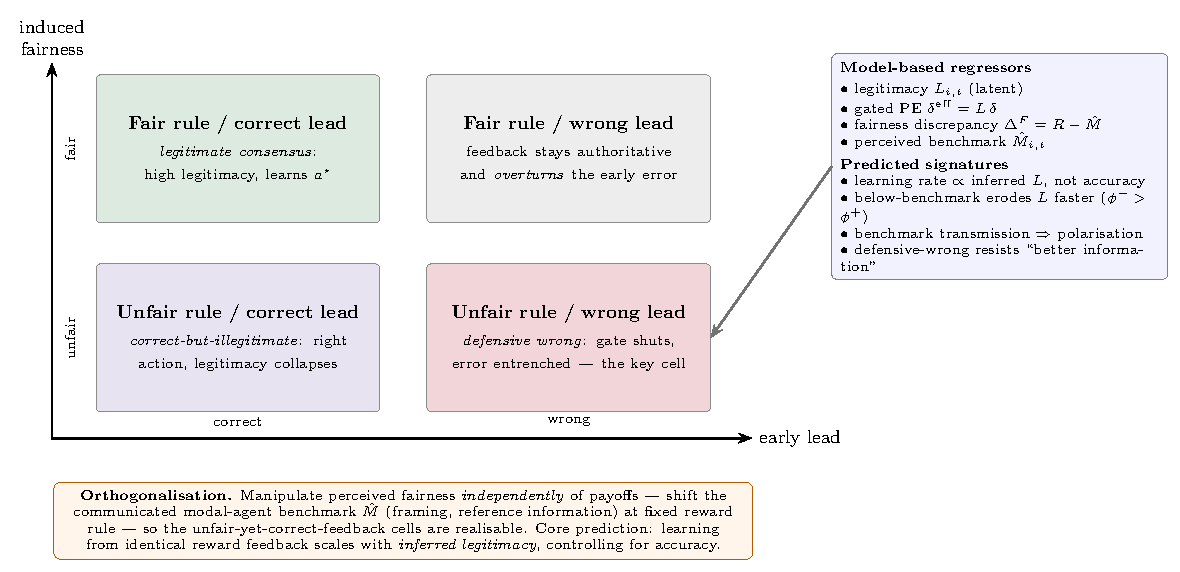
\includegraphics[width=\textwidth]{fig_experiment.pdf}
\caption{Model-based experimental design. Perceived fairness is manipulated
orthogonally to payoffs (by shifting the communicated modal-agent benchmark
$\hat M$), crossing an early lead (correct vs wrong) to realise the four regimes;
the unfair/wrong-lead cell is the falsifiable defensive-wrong prediction. The
model supplies latent regressors (legitimacy $L$, gated PE $L\delta$, fairness
discrepancy, benchmark $\hat M$) and predicted signatures for a model-based
analysis.}
\label{fig:experiment}
\end{figure}

\paragraph{Limitations.}
The baseline is deliberately narrow: binary actions, stationary rewards, fixed
networks, a single fairness benchmark (the modal-agent reward benchmark), and a
legitimacy gate on the private prediction error only. It excludes strategic
misrepresentation, endogenous rewiring, multiple competing fairness philosophies,
institutional rule change, and empirical calibration. These are natural
extensions once the minimal mechanism is fixed.

\section{Conclusion}
We have presented a self-contained model of legitimacy-gated social learning in
which reward feedback disciplines beliefs only to the extent that the reward rule
is treated as legitimate, and legitimacy is itself learned from socially
transmitted fairness benchmarks. The model produces legitimate, correct-but-
illegitimate, defensive-wrong, and fairness-polarised regimes, and shows that
legitimacy collapse turns correctable error into persistent error. A replication
package regenerates every result.

The contribution sits at the intersection of three mature literatures and adds
the connective tissue between them. From \emph{behavioural game theory} it takes
the stochastic-choice, boundedly-rational equilibrium tradition --- quantal
response and its regular form, the anomalies it was built to explain, set-valued
M-equilibrium, and level-$k$ reasoning
\citep{McKelveyPalfrey1995,GoereeHoltPalfrey2005,GoereeHolt2001,GoereeLouis2021,CrawfordCostaGomesIriberri2013}
--- and supplies the missing dynamics: the regimes here are not posited but
\emph{selected} by a gated learning process whose rest points we characterise
completely (Propositions~\ref{prop:existence}--\ref{prop:hysteresis}) and whose
collapse is a transcritical bifurcation. From the \emph{economics of fairness and
endogenous norms} it takes reference-dependent, asymmetric fairness and the
\emph{heterogeneity} of fairness ideals
\citep{FehrSchmidt1999,CharnessRabin2002,CappelenHoleSorensenTungodden2007,Andre2024ShallowMeritocracy,Bowles1998},
and makes the reference a transmissible state, so that grievance itself diffuses
on a network. The resulting fairness polarisation is a social analogue of
\emph{quasi-non-ergodicity}: like agents who trade on a public signal and
``continue to disagree forever'' \citep{BouchaudFarmer2023}, communities separated
by a benchmark gap settle into path-dependent, self-fulfilling legitimacy
regimes that history, not payoffs, selects. From \emph{neuroeconomics and
cognitive neuroscience} it takes the view of feedback whose evidential weight is
contextually modulated, positioning legitimacy on the state-representation side of
the value-versus-state debate over prefrontal computation
\citep{PadoaSchioppaConen2017,HaydenNiv2021,JoinerPivaTurrinChang2017} and casting
defensive-wrong consensus as socially-induced impairment of reversal learning
\citep{IzquierdoBrigmanRadkeRudebeckHolmes2017}. Where the field currently treats
the authority of evidence as fixed, the model makes it an endogenous, learnable,
transmissible state --- and the policy-relevant consequence is sharp:
interventions that restore accurate information do not help a community that no
longer treats information as legitimate; only interventions that restore
legitimacy reopen learning.

\appendix
\section{Proofs}
\label{app:proofs}

\begin{proof}[Proof of Proposition~\ref{prop:drift}]
Take expectations of \eqref{eq:Lupdate} ignoring the projection (valid in the
interior); the two terms are the expected erosion and recovery. The sign of the
sum determines the drift.
\end{proof}

\begin{proof}[Proof of Proposition~\ref{prop:slowdown}]
Substituting $\delta^{\mathrm{eff}}_{i,t}=\bar L\,\delta_{i,t}$ into
\eqref{eq:Qupdate}, the chosen-arm value follows
$Q_{t+1}=Q_t+\alpha\bar L\,(R-Q_t)$ on visits, a contraction toward $\E[R]$ with
modulus $1-\alpha\bar L$; the relaxation time is
$-1/\log(1-\alpha\bar L)\sim 1/(\alpha\bar L)$
\citep{SuttonBarto2018,Borkar2008}.
\end{proof}

\begin{proof}[Proof of Lemma~\ref{lem:gap}]
Apply \eqref{eq:Mupdate} to community means; the antisymmetric mode has
multiplier $(1-\psi)+\psi(B_{cc}-B_{cd})=1-2\psi\Gamma$, using
$B_{cd}=1-B_{cc}=\Gamma$ for two communities.
\end{proof}

\begin{proof}[Proof of Proposition~\ref{prop:equilibrium}]
(i) A rest point is a self-consistent choice distribution under the logistic
(quantal) map, hence a quantal-response fixed point \citep{McKelveyPalfrey1995}.
(ii) The benchmark recursion \eqref{eq:Mupdate} contracts the antisymmetric mode
by the factor $1-2\psi\Gamma$ per trial, which $\to1$ as $\psi\Gamma\to0$, so a
benchmark gap persists and the two communities settle at different
(choice, benchmark) pairs; monotone choices together with community-specific
self-consistent beliefs are the defining conditions of M-equilibrium
\citep{GoereeLouis2021}. Convergence of the finite-$N$ ensemble to these rest
points is the standard stochastic-approximation limit \citep{Borkar2008}.
\end{proof}

\begin{proof}[Proof of Proposition~\ref{prop:existence}]
The choice probability is a continuous (logistic) function of the values, the
expected gated value increment and the expected legitimacy increment are
continuous in $(Q,L)$, and the projection onto $[0,1]$ is continuous; hence
$T_{\hat M}$ maps the compact convex set $[0,1]^2\times[0,1]$ continuously into
itself and Brouwer's theorem gives a fixed point. At a fixed point the value
equation reads $L^\star\,\1\{A=a\}\,(\E[R\mid a]-Q^\star(a))=0$ for each arm; if
$L^\star>0$ this forces $Q^\star(a)=\mu_a$ on visited arms, so
$\Delta^\star=\mu_{a^\star}-\mu_o$ and the choice is the quantal response to
$\Delta^\star$, while at $L^\star=0$ the increment vanishes and $Q^\star$ may be
frozen. The value coordinate is thus monostable for $L^\star>0$, and the
equilibria are indexed by the legitimacy roots analysed in
Proposition~\ref{prop:hysteresis}.
\end{proof}

\begin{proof}[Proof of Proposition~\ref{prop:hysteresis}]
At the value nullcline the choice distribution is fixed, so
$\bar D^F(\hat M)$ and hence the tilt $h(\hat M)$ are constants and \eqref{eq:cusp}
is an autonomous scalar cubic. Interior equilibria solve $g(x):=x^3-(r/s)x-(h/s)=0$.
The depressed cubic $x^3+px+q$ with $p=-r/s<0$, $q=-h/s$ has three distinct real
roots iff its discriminant is positive, $4p^3+27q^2<0$, i.e.\
$(h/s)^2<\tfrac{4}{27}(r/s)^3$, equivalently $|h|<h_c=2s\,(r/(3s))^{3/2}$; it has
one real root when $|h|>h_c$ and a double root at $|h|=h_c$. A scalar rest point
$x^\star$ is asymptotically stable iff $\dot x'(x^\star)=r-3s\,x^{\star2}<0$; the
two outer roots satisfy this and the middle root does not, giving two stable wells
and one saddle in the bistable band. As $\hat M$ varies, $h(\hat M)$ crosses
$\pm h_c$, where a stable root and the saddle coalesce and annihilate --- a
saddle-node (fold). The two folds bound a bistable interval over which the
attained equilibrium depends on the initial condition, which is hysteresis (the
cusp normal form). Finally, letting the wells' curvature diverge so that the
stable roots are driven to the boundaries recovers the additive, hard-clipped
limit, in which the pair of folds degenerates to the single boundary transcritical
at $\hat M^\star=(\tau^F+\nu_R\mu_{a^\star}/[\nu_F(1-\mu_{a^\star})])/\phi^-$
(the balance point of Proposition~\ref{prop:drift}).
\end{proof}

\section{ODD+D description}
\label{app:odd}

\paragraph{A.1 Purpose and patterns.}
To determine when reward feedback stops being treated as valid evidence because
the rule is perceived as unfair, and how network geometry shapes the result.
Target patterns: \textbf{P1} legitimate consensus; \textbf{P2}
correct-but-illegitimate consensus; \textbf{P3} defensive wrong consensus
(legitimacy collapse making a correctable error persistent); \textbf{P4} fairness
polarisation under identical payoffs; \textbf{P5} an acceptability-threshold
transition; \textbf{P6} geometry-controlled benchmark diffusion. Not targeted:
empirical fairness time-series, continuous actions, non-stationary rules.

\paragraph{A.2 Entities, state variables, scales.}
Agents (values $Q_{i,t}(a)$, confidence $C_{i,t}$, legitimacy $L_{i,t}$, perceived
benchmark $\hat M_{i,t}$), communities, two arms, and a row-stochastic coupling
matrix $B$. Time is discrete at the trial level with horizon $T$.

\paragraph{A.3 Process overview and scheduling.}
Synchronous trials with a simultaneous update: (1) credibility field from the
previous period; (2) augmented values; (3) process-based choice and confidence;
(4) reward; (5) fairness discrepancy, discomfort and legitimacy update from the
pre-update state; (6) legitimacy-gated private plus retrospective-social value
update; (7) modal-agent benchmark update; (8) record.

\paragraph{A.4 Design concepts.}
\emph{Basic principles:} prediction-error learning gated by legitimacy; fairness
judged against a social benchmark. \emph{Emergence:} regimes from rules and
coupling. \emph{Adaptation:} gated value revision and legitimacy/benchmark
learning. \emph{Objectives:} myopic reward through learned values.
\emph{Sensing:} neighbours' actions, confidence and benchmarks; own reward vs
benchmark. \emph{Interaction:} weighted by $B$ and credibility.
\emph{Stochasticity:} choice and Bernoulli rewards. \emph{Collectives:}
communities. \emph{Observation:} the observables of Section~\ref{sec:design}.

\paragraph{A.5 Initialisation.}
Community-constant initial values, legitimacy $L_0$ and benchmarks $\hat M_0$ per
Table~\ref{tab:params} and the per-experiment scenarios; benchmark disagreement is
set through $\hat M_0=(0.5\mp|\Delta\hat M_0|/2)$.

\paragraph{A.6 Input data.} None; the model is synthetic.

\paragraph{A.7 Submodels.} Credibility field; augmented value and choice;
confidence; fair benchmark $r^F=f(a,\hat M)$; fairness discrepancy
\eqref{eq:dF}; asymmetric discomfort \eqref{eq:DF}; legitimacy update
\eqref{eq:Lupdate}; legitimacy-gated prediction error \eqref{eq:gate}; value
update \eqref{eq:Qupdate}; modal-agent transmission \eqref{eq:Mupdate}; regime
classifier. Each maps to code and a test in the ODD-to-code map
(\texttt{ODD\_to\_code\_map.md}).

\paragraph{A.8 Parameters.} Global defaults in Table~\ref{tab:params};
per-experiment values in \texttt{scenarios.py}.

\paragraph{A.9 Code-location map.} See \texttt{ODD\_to\_code\_map.md}: each
equation maps to a function in \texttt{code/legitimacy/} and a check in
\texttt{tests/test\_legitimacy.py}.

\paragraph{A.10 Verification and reproducibility.} Appendix~\ref{app:tests} and
the replication metadata; all results regenerate from seeded scripts.

\section{Verification}
\label{app:tests}
The implementation passes an automated suite of $11$ checks (all green):
legitimacy and value bounds in $[0,1]$; the effective-prediction-error identity
$\delta^{\mathrm{eff}}=L\delta$ (and $L\equiv1$ when the gate is off); the
discomfort asymmetry ($\phi^->\phi^+\Rightarrow$ larger legitimacy loss for
disadvantageous unfairness); the acceptability-threshold partition; modal-agent
misperception (a benchmark gap persists under low permeability and erodes under
full mixing); modal-agent bounds (including idiosyncratic noise); exactness of
the balanced-block community field for the modal-agent update; the regime
classifier on hand-built inputs; seed reproducibility; the no-gate ablation
(removing the gate restores correction of an early wrong lead); and the
true-benchmark ablation (pinning $\hat M=M$, and the effort-reward benchmark
form).

\section{Parameters}
\label{app:params}
% Auto-generated -- default parameters.
\begin{table}[t]\centering\small
\caption{Global default parameters (\texttt{code/legitimacy/config.py}); per-experiment values are in \texttt{scenarios.py}. Values are projected to $[0,1]$; the fairness-in-choice term is off by default.}
\label{tab:params}
\begin{tabular}{llll}\toprule
Symbol & Default & Role & Config key \\ \midrule
$\mu_1,\mu_2$ & 0.6,0.4 & arm reward means & \texttt{mu} \\
$\lambda$ & 0.5 & anticipatory weight & \texttt{lam} \\
$\eta$ & 0.2 & retrospective weight & \texttt{eta} \\
$\beta,\sigma,a$ & 6.0,1.0,1.0 & DDM choice & \texttt{beta,sigma,a\_thr} \\
$\alpha$ & 0.2 & private learning rate & \texttt{alpha} \\
$\nu_F,\nu_R$ & 0.05,0.01 & legitimacy loss / recovery & \texttt{nu\_F,nu\_R} \\
$\tau^F$ & 0.3 & acceptability threshold & \texttt{tau\_F} \\
$\phi^-,\phi^+$ & 1.0,0.25 & discomfort weights ($\phi^->\phi^+$) & \texttt{phi\_minus,phi\_plus} \\
$\psi$ & 0.1 & modal-agent transmission & \texttt{psi} \\
$L_0$ & 1.0 & initial legitimacy & \texttt{L0} \\
\bottomrule\end{tabular}
\end{table}

Per-experiment scenario parameters (population size, horizon, replications,
$\lambda$, $\eta$, $\nu_F$, $\nu_R$, $\tau^F$, $\hat M_0$, initial values and
seeds) are defined in \texttt{code/legitimacy/scenarios.py}, the authoritative
source, and summarised in \texttt{reports/replication\_audit.md}.

\section{Robustness}
\label{app:robust}
The qualitative regimes are stable to the terminal threshold and to moderate
changes in the discomfort weights and loss/recovery rates around the values in
Table~\ref{tab:params}; the legitimacy-collapse boundary follows
Proposition~\ref{prop:drift}. A systematic robustness sweep (threshold, horizon,
benchmark strength, permeability, and a graph-perturbation check analogous to the
credibility baseline) is the immediate next step and is scaffolded in
\texttt{reports/robustness\_summary.md}.

\bibliographystyle{apalike}
\bibliography{legitimacy_fairness}
\end{document}
